\chapter{Exact intensity for the two-faceted cup}\label{app:boundariescup}
For very simple optical systems, the \textit{exact} target intensity of light emitted from the source and propagating within the system can be calculated. Here we explain how this is done for the two faceted cup formed by a Lambertian source described in Chapter \ref{chap:raytracing}. We remind the reader that, for this system, the intensity in a given distance $\variabile{p}$ in PS is defined as:
\begin{equation}\label{eq:eta_appendix}
I_{\textrm{PS}}(\variabile{p}) = \sum_{\Pi}\int_{\variabile{q}^\textrm{\,min}(\Pi, \variabile{p})}^{\variabile{q}^\textrm{\,max}(\Pi,\variabile{p})}L(\variabile{q}, \variabile{p})\textrm{d}\variabile{q} = \sum_{\Pi}\big (\variabile{q}^\textrm{max}(\Pi,\variabile{p})-\variabile{q}^\textrm{\,min}(\Pi,\variabile{p})\big )\,,
\end{equation}
where the sum is over all the possible paths and the second equation holds as we assume $L=1$ in \insieme{R}$_\textrm{t}(\Pi)$ and, $\variabile{q}^\textrm{\,min}(\Pi,\variabile{p})$ and $\variabile{q}^\textrm{\,max}(\Pi,\variabile{p})$ are the minimum and maximum position coordinates of the rays on $\partial$\insieme{R}$_\textrm{t}(\Pi)$ along direction $\variabile{p}$. Therefore, if we are able to provide an analytic expression for the boundaries $\partial$\insieme{R}$_\textrm{t}(\Pi)$ we can calculated the position coordinates $\variabile{q}^\textrm{\,min}(\Pi,\variabile{p})$ and $\variabile{q}^\textrm{\,max}(\Pi,\variabile{p})$ of the intersection points between line $\variabile{p}=\textrm{const}$ and $\partial$\insieme{R}$_\textrm{t}(\Pi)$ analytically from which the exact intensity for every direction $\variabile{p}$ is obtained using Equation (\ref{eq:eta_appendix}). The procedure used for such purpose is explained next.
\section{Analytic boundaries calculation}
The idea is to rotate the cup to determine the maximum number of reflections between the rays and the optical lines before reaching the target. The rays are considered to be straight lines instead of broken lines. Hence it is sufficient to find only one intersection point between the ray and a line segment (also in the case where we have more than one reflection occur). Finally rotating back these point we obtain the corresponding coordinates at the target.\\ \indent
Next we explain this procedure in detail.
The two-faceted cup is defined in the $(\variabile{x}, \variabile{z})$ plane as in Chapter \ref{chap:raytracing}. 
Let $\gamma$ be the angle that the left and right reflector make with the normal to the source measured conterclockwise. 
%\begin{figure}[t]
%\label{fig:cup}
%  \begin{center}
%%\vspace{-1.5cm}
%  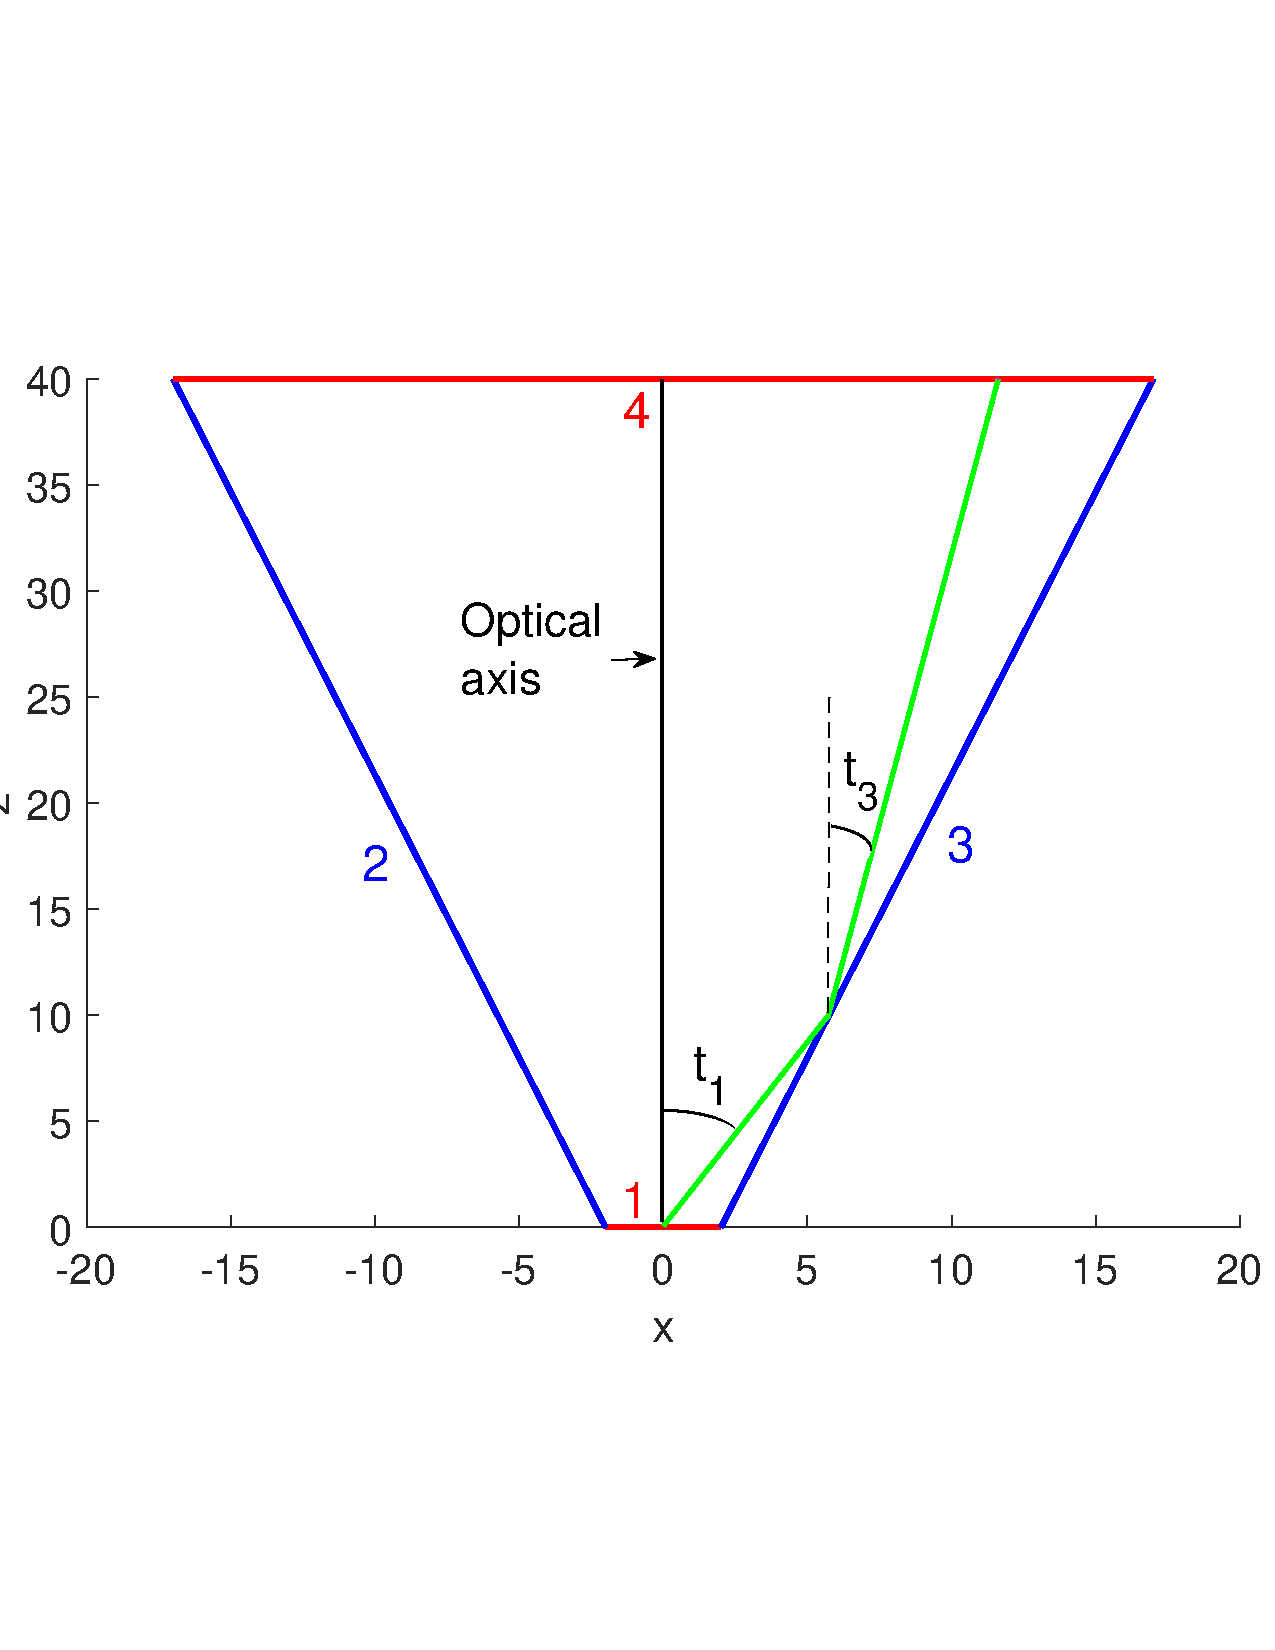
\includegraphics[width=6.7cm]{cup.pdf}
%  \end{center}
%%\vspace{-2cm}
%  \caption{\textbf{Shape of the two-faceted cup.}  Each line of the system is labeled with a number.
%   The source \point{S}$= [-2,2]$ (line number $1$) is located on the $\variabile{x}$-axis.
%   The target \point{T}$= [-17, 17]$ (line $4$) is parallel to the source and is located at a height $\variabile{z}= 40$.
%   The left and right reflectors (line $2$ and $3$) connect the source with the target.}
%  \label{fig:cup}
%\end{figure}
The highest $\variabile{z}$ coordinate $C$ that the two-faceted cup can reach during the rotation is defined by:
\begin{equation}\label{rotation}\begin{tabular}{llll}
$C$ & $=$ & $ \big(h+\frac{\variabile{a}}{\tan\gamma}\big)\frac{1}{\cos\gamma}-\frac{\variabile{a}}{\tan\gamma}$ \\ $ \quad$ & $ \quad $ & $ \quad $ \\$ \quad$ &  $=$ & $\frac{h}{\cos\gamma}+a\tan\big(\frac{1}{2}\gamma\big),$\end{tabular}
\end{equation} and $\point{B}=(0,C)$ is the rotation point. We define $\point{B}_k$ as the clockwise ($k<0$) or counterclockwise ($k\geq 0$) rotations of the point $\point{B}=(0,C)$ over an angle $\alpha_k=(2k+1)\gamma$, with $k$ an integer number (Figure $\ref{fig:twofaced}$ is illustrative).
\begin{figure}[t]%\label{fig:twofaced}
 \begin{center}
  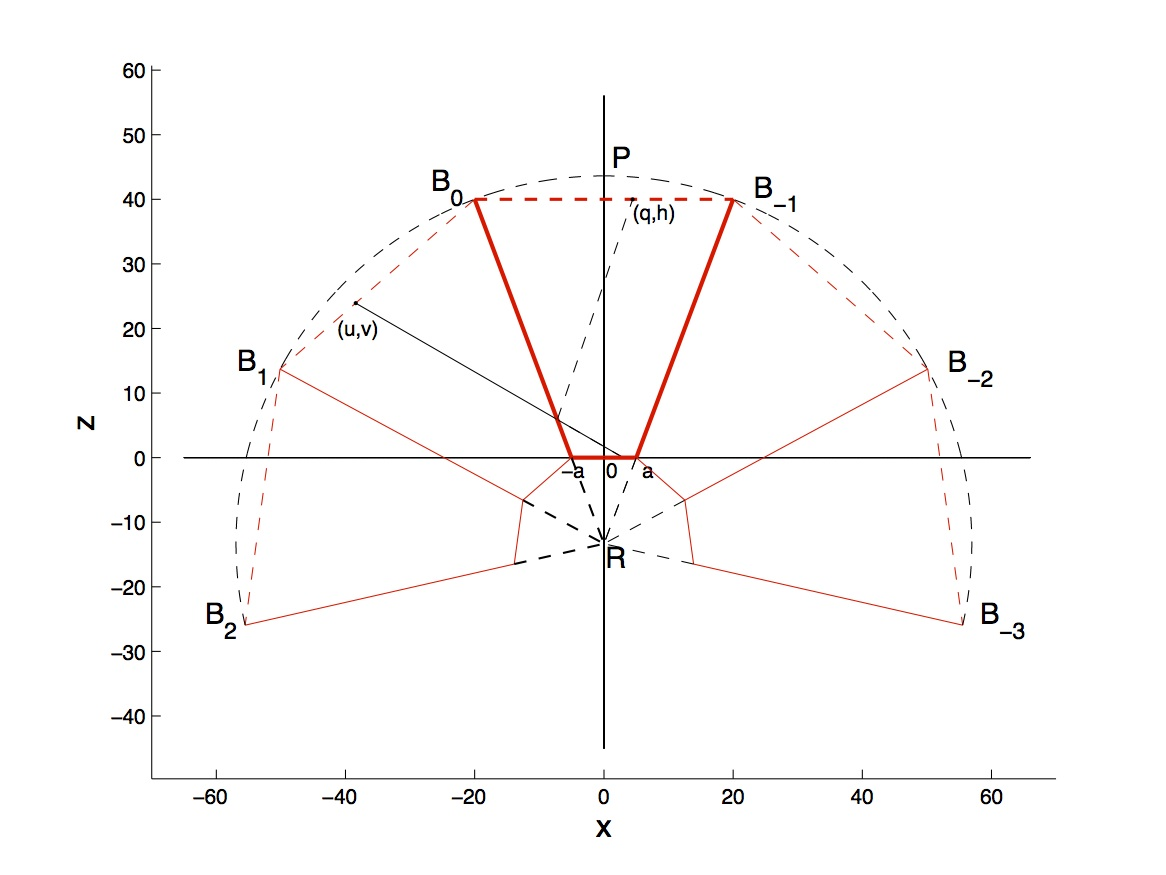
\includegraphics[width=10cm]{rotatedcup.jpg}
  \end{center}
 \caption{\textbf{The two-faceted cup rotated twice on both sides.} The line segment with end points $B_{k-1}$ and $B_{k}$ is the $|k|$ times rotated target. Rotating the coordinates $(u,v)$ of the intersection point between a ray and the segment $B_0B_1$ the coordinates $(q,h)$ on the target $B_{-1}B_{0}$ are obtained. The point $\point{R} = \big(0,-\frac{a}{\tan{\gamma}}\big)$ is the center of the circle described by rotating the cup (dashed line).}
  \label{fig:twofaced}
  \end{figure}
  %as the notation used in equation ($\ref{Bk}$) could suggest.
The position coordinates of points $\point{B}_k = (B_{k,x}, B_{k,z})$ are given by:
\begin{equation}
 \begin{pmatrix} B_{k,x}  \\  B_{k,z}\end{pmatrix}= -
  \begin{pmatrix} 0  \\  \frac{a}{\tan\gamma}\end{pmatrix}+
 \left(\begin{split}  & \cos\alpha_k  & -\sin\alpha_k \\  & \sin\alpha_k & \cos\alpha_k\end{split}\right)
 \begin{pmatrix}  0 \\  C+\frac{a}{\tan\gamma}\end{pmatrix},
\end{equation}
The maximum number of reflections $r_{\textrm{max}}$ a ray can undergo before arriving at the target is:
\begin{equation}
r_{\textrm{max}}=\max\{k\in\mathbb{N} \;| \; B_{k-1,z}\geq 0\}.
\end{equation}
For the two-faceted cup depicted in Figure \ref{fig:cup} we found $r_{\textrm{max}}=2$.\\ \indent 
Given the position coordinates $(\variabile{x}_1, \variabile{z}_1)$ and the angular coordinate $\optangle_1$ of a ray at the source we can calculate the corresponding position $(\variabile{x}, \variabile{z})$ and direction $\optangle$ coordinates at the target as explained in the following. \\ \indent We compute the coordinates $(u,v)$ of the intersection point between the ray parametrization and the $\variabile{k}$ times mirrored target $\point{B}_{\variabile{k}-1}\point{B}_\variabile{k}$ for which the intersection with the forward ray is not empty where $\variabile{k}=-\variabile{r}_{\textrm{max}}-1, \cdots, \variabile{r}_{\textrm{max}}$. Next, if $\variabile{k}$ is even, the corresponding coordinates $(\variabile{x},\variabile{z})$ at the target are found by rotating back the coordinates $(\variabile{u},\variabile{v})$, otherwise a reflection is applied.\\ \indent
The method of reflecting the cup instead of the rays allows to determine the positive luminance regions $\big(\mbox{\insieme{R}}_(\Pi_{\variabile{j}})\big)_{\variabile{j}=1, \cdots, 2\variabile{k}+1}$ in target PS, where every path $\Pi_{\variabile{j}}$ corresponds to a certain number $\variabile{k}$ of reflections. The set of rays that form the boundaries $\partial$\insieme{R}$(\Pi_{\variabile{j}})$ only consists of rays that either leave the extremes of the source or hit one of the points $\point{B}_\variabile{k}$. At the boundaries a small change in the position or direction ray coordinate can cause a difference in the number of the reflections. The angular coordinates of the rays that leave the point of the source with coordinate $(\variabile{x}_1, \variabile{z}_1)$ and hit $\point{B}_\variabile{k}$ are given by:
\begin{equation}\label{anglesource}
\tan \optangle_1 = \frac{\variabile{x}_1-B_{k,x}}{B_{k,z}}.
\end{equation}
Note that the rays emitted from the end points of the source form vertical lines in source PS \insieme{S} because $\variabile{x}_1 = \textrm{const}$. On the other hand, rays that hit points $\point{B}_k$ form vertical lines in target PS \insieme{T} as $\varaibile{x}_4 = \textrm{const}$.

Therefore, the ray coordinates $(\variabile{x},\variabile{z})$ at the target are given by:
\begin{equation} \label{rotation_target}\begin{pmatrix} \variabile{x}\\ \variabile{z}
\end{pmatrix} = \left(\begin{array}{cc}(-1)^k & 0  \\ 0 & 1\end{array}\right)
\left(\begin{array}{cc}\cos(-2\variabile{k}\gamma) & -\sin(-2\variabile{k}\gamma) \\\sin(-2\variabile{k}\gamma) & \cos(-2\variabile{k}\gamma)\end{array}\right)\begin{pmatrix} \variabile{u} \\
 \variabile{v}+\frac{a}{\tan(\gamma)}\end{pmatrix}-\begin{pmatrix}0 \\ \frac{a}{\tan\gamma}\end{pmatrix}.
\end{equation} We observe that the sign depends on the parity of $\variabile{k}$. When $\variabile{k}=0$, i.e. the ray does not reflect, the first and the second matrices become the identity matrix and the cup is not rotated nor reflected. When $\variabile{k}$ is even, the determinant of the matrix given by the product between the first and the second matrix ($\ref{rotation_target}$) is equal to $1$ and we obtained a rotation matrix, while when $\variabile{k}$ is odd the determinant of the product matrix is $-1$ and we have a reflection matrix.
Also the angle on the target is calculated. It is an addition of an angle and a change of sign depending on $\variabile{k}$:
\begin{equation}\label{teta}
\theta=(-1)^\variabile{k}(t-2\variabile{k}\gamma).
\end{equation}






This method of rotating the cup instead of reflecting the ray inside the system can also be applied to find the boundaries of the regions
$M_{\textrm{s},k}$ and $M_{\textrm{t},k}$. In the following sections we will illustrate how this is done.
\\




\subsection{Source phase space}
We observe that the set of rays that form the boundary of the regions $M_{\textrm{s},k}$ only consists of rays that either leave the extremes of the source or hit one of the points
$B_k$. In Figure $\ref{fig:twofaced}$ is shown a ray that on the target phase space is located inside the region
$M_{\textrm{t},1}$, it does not constitute a point on any boundary. 
Hence for the representation on the source phase space we have to choose rays that hit $ B_{k} $, their directions are given by the relation \begin{equation}\label{anglesource}
\tan t = \frac{x-b_{k,x}}{b_{k,z}}\,.
\end{equation}
This is exactly what we did in the algorithm named \textit{'Source'} (see Appendix \ref{sec:source} for details).
\begin{figure}
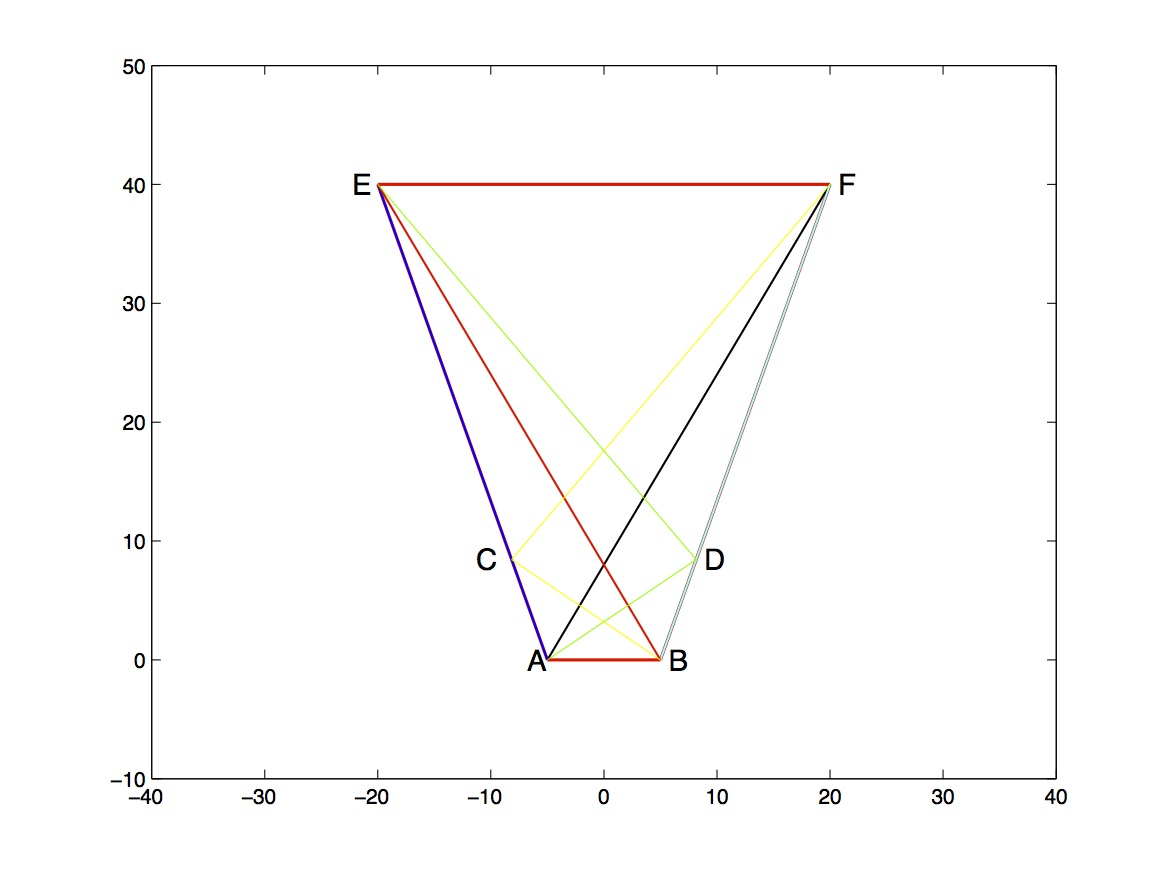
\includegraphics[scale=0.55]{raggi6.jpg}
\caption{\footnotesize{Rays that leave the corner points of the source. The rays $AF$, $BE$, $ACE$, $BDF$ are rays that do not hit the reflectors of the system.
They constitute rays on the boundaries of the regions $M_{\textrm{s},0}$, $M_{\textrm{s},1}$ and $M_{\textrm{s},-1}$.
 The rays $ADE$ and $BCF$ are rays that hit once the reflectors of the system. They constitute rays on the boundaries of the regions
 $M_{\textrm{s},-1}$, $M_{\textrm{s},-2}$, and $M_{\textrm{s},1}$ or $M_{\textrm{s},2}$, respectively.}}
\label{fig:raggi}
%\end{minipage}
\end{figure}

\begin{figure}[htbp]
%\centering
%\begin{minipage}[t]{.40\textwidth}
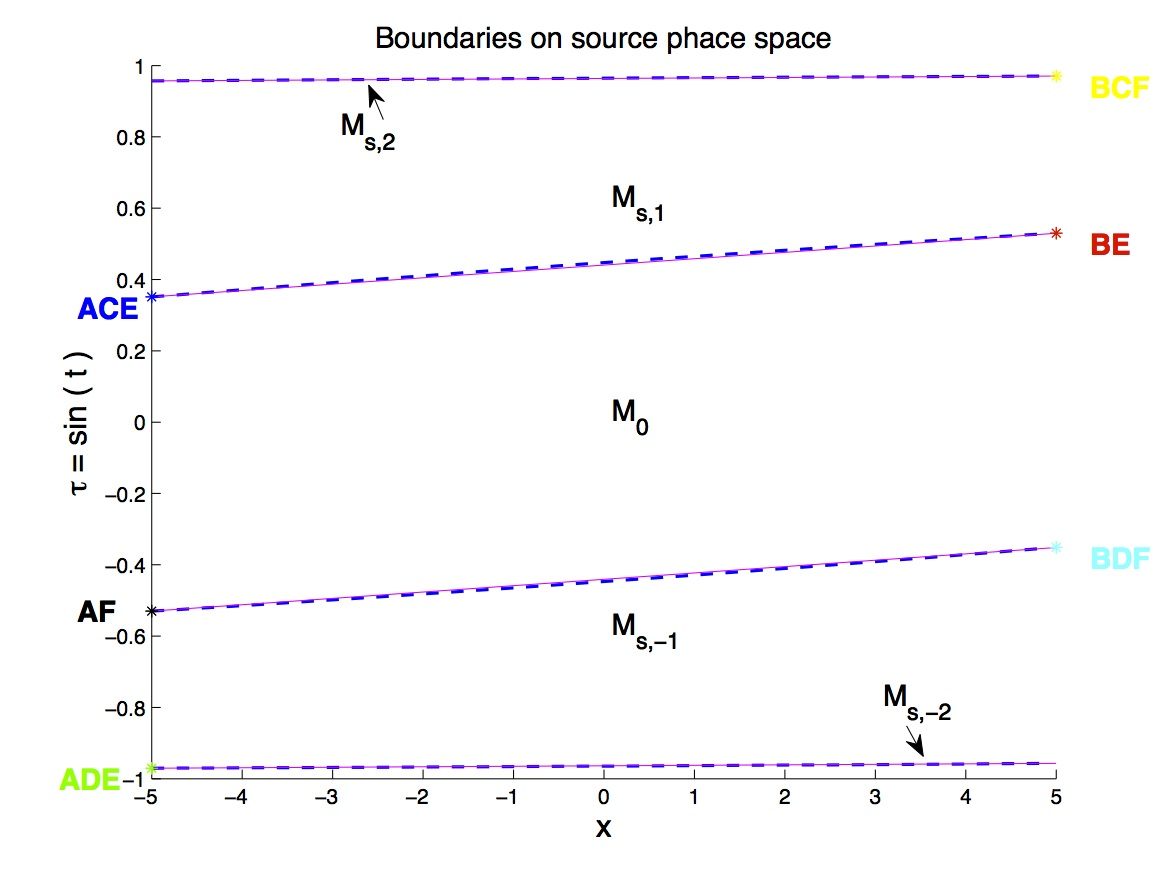
\includegraphics[scale=0.55]{boundaries_source.jpg}
\caption{\footnotesize{Regions $M_{s,k}$ of rays that reflect $|k|$ times, with $(x,\tau)\in\mathcal{P}_\textrm{s}$.
The parameter values are: $a=5$, $b=20$ and $h=40$. The continuous lines are the boundaries of the regions $M_{\textrm{s}}$
calculated considering rays that leave the source and hit the points $B_{k}$ at the target. The dashed blue lines are the boundaries calculated using ($\ref{anglesource}$) }}
\label{fig:boundary}
%\end{minipage} \qquad \qquad
%\begin{minipage}[t]{.40\textwidth}
\end{figure}
In Figure $\ref{fig:raggi}$ are shown some rays that compose the boundaries of $M_{\textrm{s},k}$ which coordinates are:
$$ \begin{array}{cc}ADE = \Bigg(-a, \arctan\Big(\frac{-a+b_{-1,x}}{b_{-1,z}}\Big)\Bigg),\; ACE = \big(-a, \sin(\gamma)\big),\; AF = \big(-a, -\sin(\delta)\big), \\
 BCF = \Bigg(a, \arctan\Big(\frac{a-b_{1,x}}{b_{1,z}}\Big)\Bigg), BDF = \big(a, - \sin(\gamma)\big) \, \;\mbox{and} \,\; BE = \big(a, \sin(\delta)\big).\end{array} $$
The rays are represented by points in phase space.
So we choose a proper number of rays that leave the source to obtain an accurate representation of the boundaries of  $M_{\textrm{s},k}$ regions.
The final result is shown in Figure $\ref{fig:boundary}$.
In addition, we derive the exact equation for the map $\mathcal{M}$.
From equation ($\ref{anglesource}$) we find the value of the angle for each ray at the source (depending on the ray position).
Thus the boundaries are simply straight lines in the $(x, \tan(t))$-plane. The subdivision of phase space into regions is shown in Figure
%Hence, on source phase space, the boundaries of the regions formed by rays that reflect $|k|$ times are given by the functions \begin{equation}\begin{matrix}
%f_{k} \colon &  [-a,a]  & \to  & [-1, 1]  \\   \mbox{ } &  x & \mapsto &    \sin(t)
% \end{matrix} \end{equation} such that:
%\begin{equation}\label{analytic}
%f_{k}(x) = \sin\Bigg(\arctan\bigg(\frac{x-b_{k,x}}{b_{k,z}}\bigg)\Bigg)\,.
%\end{equation}
$\ref{fig:boundary}$, where we can also see the comparison between the two different methods to calculate the boundaries. Note that in this specific case the boundaries appear straight lines also in the $(x,sin(t))$-plane.
%\newpage
\subsection{Target phase space}
In this section we derive an exact expression for the map $\mathcal{M}$ in such a way that it is possible to determine the boundaries of the regions $M_{\textrm{t},k}$
simply by finding the images of some points on $\partial M_{\textrm{s},k}$.
Given a ray parameterization we are able to calculate the intersections point $(u,v)$ between the ray and the line segment $B_{k-1}B_{k}$ as we did in \textit{'Target'} (See Appendix \ref{sec:target} for the procedure).
 The corresponding point $(q,h)$ on the target can be found by rotating or reflecting the point $(u,v)$ back for $k$ even or odd, respectively.
 Therefore we have the following expression for the point $(q,h)$ on the target:
\begin{equation} \label{rotation_target}\begin{pmatrix} q\\ h
\end{pmatrix} = \left(\begin{array}{cc}(-1)^k & 0  \\ 0 & 1\end{array}\right)
\left(\begin{array}{cc}\cos(-2k\gamma) & -\sin(-2k\gamma) \\\sin(-2k\gamma) & \cos(-2k\gamma)\end{array}\right)\begin{pmatrix} u \\
 v+\frac{a}{\tan(\gamma)}\end{pmatrix}-\begin{pmatrix}0 \\ \frac{a}{\tan(\gamma)}\end{pmatrix}\,.
\end{equation} We observe that the sign depends on the parity of $k$. When $k=0$, i.e. the ray does not reflect, the first and the second matrices become the identity matrix and the cup is not rotated nor reflected. When $k$ is even, the determinant of the product between the first and the second matrixes at the right hand of equation ($\ref{rotation_target}$) is equal to $1$ and we obtained a rotation matrix, while when $k$ is odd the determinant of the matrix given by the product between the first and the second matrix is equal to $-1$ and we have a reflection matrix.
Also the angle on the target is calculated. It is an addition of an angle and a change of sign depending on $k$:
\begin{equation}\label{teta}
\theta=(-1)^k(t-2k\gamma).
\end{equation}
For every $k$, the mapping $(x,t)\mapsto(q,\theta)$ is now well determined and also the regions $M_{\textrm{s},k}$ of rays that reflect $k$ times are mapped to $M_{\textrm{t},k}$.
We observe that the lines shown if Figure $\ref{fig:boundary}$ are mapped to vertical lines in target phase space by the map $\mathcal{M}$ (see Figure \ref{boundaries_target}).  Hence, to obtain the boundaries of the target,we will choose rays that are emitted from points close to the boundary of the source.
According to what we said so far, the case of the target requires some good calculation to determine where a ray exits the cup.
We can obtain those points analytically for a suitable number of rays, as we did in \textit{'Target'}, and then we can drawn those points on the phase space as is shown in
Figure $\ref{boundaries_target}$.

 \begin{figure}[htbp]
%\centering
%\begin{minipage}[t]{.40\textwidth}
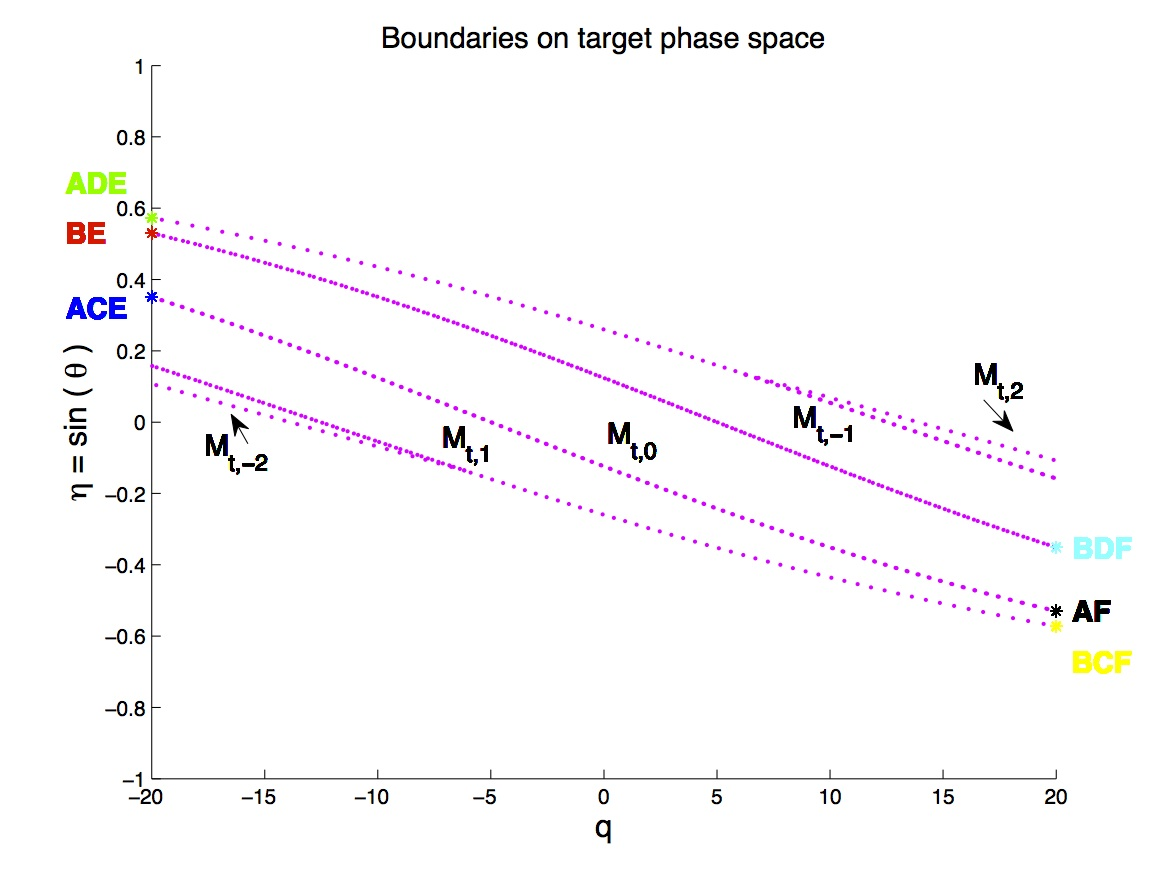
\includegraphics[scale=0.55]{boundaries_target.jpg}
\caption{Regions $M_{t,k}$ of rays that reflect $|k|$ times, for the two-faceted cup. The parameter values are: $a=5$, $b=20$ and $h=40$.}
\label{boundaries_target}
%\end{minipage} \qquad \qquad \qquad
\end{figure}
\noindent The coordinates of the rays traced in Figure $\ref{fig:raggi}$ at the target are given by:
$$ \begin{array}{cc}ADE = \big(-b, -(t_1+2\gamma)\big)),\; ACE = \big(-b, \sin(\gamma)\big),\; AF = \big(-b, -\sin(\delta)\big), \\
 BCF = \big(b, -(t_2-2\gamma)\big), BDF = \big(b, - \sin(\gamma)\big) \, \;\mbox{and} \,\; BE = \big(b, \sin(\delta)\big).\end{array} $$
 where $t_1 = \arctan(\frac(-a+b_{-1,x}{b_{-1}}))$ and $t_2 = \arctan(\frac(a-b_{-1,x}{b_{-1}}))$.


Figure $\ref{fig:boundary}$ and $\ref{boundaries_target}$ show also the symmetry of the regions $M_{\textrm{s},k}$ and $M_{\textrm{t},k}$. Finally we note that, since $k = 1$ is odd, the position of the regions $M_{\textrm{t},1}$ and $ M_{\textrm{t},-1}$ are exchanged with respect to the position of $ M_{\textrm{s},1}$ and $ M_{\textrm{s},-1}$.
